\documentclass{article}
\usepackage{graphicx}
\usepackage{amsmath}
\usepackage{booktabs} % For better table lines
\usepackage{adjustbox} % To fit table if needed
% Packages for enhanced functionality
\usepackage{graphicx}      % For including images
\usepackage{caption}       % For customizing captions
\usepackage{amsmath}       % For mathematical symbols and environments
\usepackage{geometry}      % To adjust page margins
\usepackage{float}         % For improved figure placement
\usepackage{hyperref}      % For hyperlinks within the document

\title{Project 1 - Part 2}
\author{Adil Hydari}
\date{\today}
\begin{document}
	
	\maketitle
	\section{Lab 1}
	\subsection{Part 1}
	
	\begin{table}[ht]
		\centering
		\begin{adjustbox}{max width=\textwidth}
			\begin{tabular}{|l|c|c|c|c|c|c|c|}
				\hline
				\textbf{Benchmark}      & \textbf{Total \# of Instructions} & \textbf{Load \%} & \textbf{Store \%} & \textbf{Uncond Branch \%} & \textbf{Cond Branch \%} & \textbf{Integer Computation \%} & \textbf{Floating pt Computation \%} \\ \hline
				anagram.alpha           &25,597,771&25.36&9.93&4.46&10.30&44.63&5.31 \\ \hline
				go.alpha                &545,812,145&30.62&8.17&2.58&10.96&47.64&0.03 \\ \hline
				compress.alpha          &88,337&1.66&79.05&0.19&5.78&13.30&0.00      \\ \hline
				gcc.alpha               &337,341,325& 24.67&11.47&4.12&13.33&46.30&0.11 \\ \hline
			\end{tabular}
		\end{adjustbox}
		\caption{Instruction breakdown for given benchmarks}
	\end{table}
	
\subsection{Part 2}
	\begin{table}[ht]
	\centering
	\begin{adjustbox}{max width=\textwidth}
		\begin{tabular}{|l|c|c|c|c|c|c|c|}
			\hline
			\textbf{Alpha Benchmark}      & \textbf{Total \# of Instructions} & \textbf{Load \%} & \textbf{Store \%} & \textbf{Uncond Branch \%} & \textbf{Cond Branch \%} & \textbf{Integer Computation \%} & \textbf{Floating pt Computation \%} \\ \hline
			test.math          &49,604&17.24&10.38&3.92&11.16&55.27&1.87 \\ \hline
			test.fmath                &19,693&17.88&12.40&4.65&11.50&53.00&0.42 \\ \hline
			test.llong          &10,821&18.09&14.33&5.32&12.78&49.19&0.10      \\ \hline
			test-printf               &983,667& 18.00&10.73&4.82&11.39&54.84&0.09 \\ \hline
		\end{tabular}
	\end{adjustbox}
	\caption{Instruction breakdown for Alpha benchmarks}
\end{table}

\begin{table}[ht]
	\centering
	\begin{adjustbox}{max width=\textwidth}
		\begin{tabular}{|l|c|c|c|c|c|c|c|}
			\hline
			\textbf{Pisa Benchmark}      & \textbf{Total \# of Instructions} & \textbf{Load \%} & \textbf{Store \%} & \textbf{Uncond Branch \%} & \textbf{Cond Branch \%} & \textbf{Integer Computation \%} & \textbf{Floating pt Computation \%} \\ \hline
			test.math          &213,745&15.96&10.66&4.22&13.85&54.42&0.88 \\ \hline
			test.fmath                &53,504&16.14&14.41&4.24&15.11&49.95&0.11 \\ \hline
			test.llong          &29,687&16.33& 17.99&4.37&15.45&45.82&0.00      \\ \hline
			test-printf               &1,813,937&19.22&9.28&5.13&17.01&49.33&0.01 \\ \hline
		\end{tabular}
	\end{adjustbox}
	\caption{Instruction breakdown for Pisa benchmarks}
\end{table}
\subsection{Comparison with Histogram}
\begin{figure}[H]
	\centering
	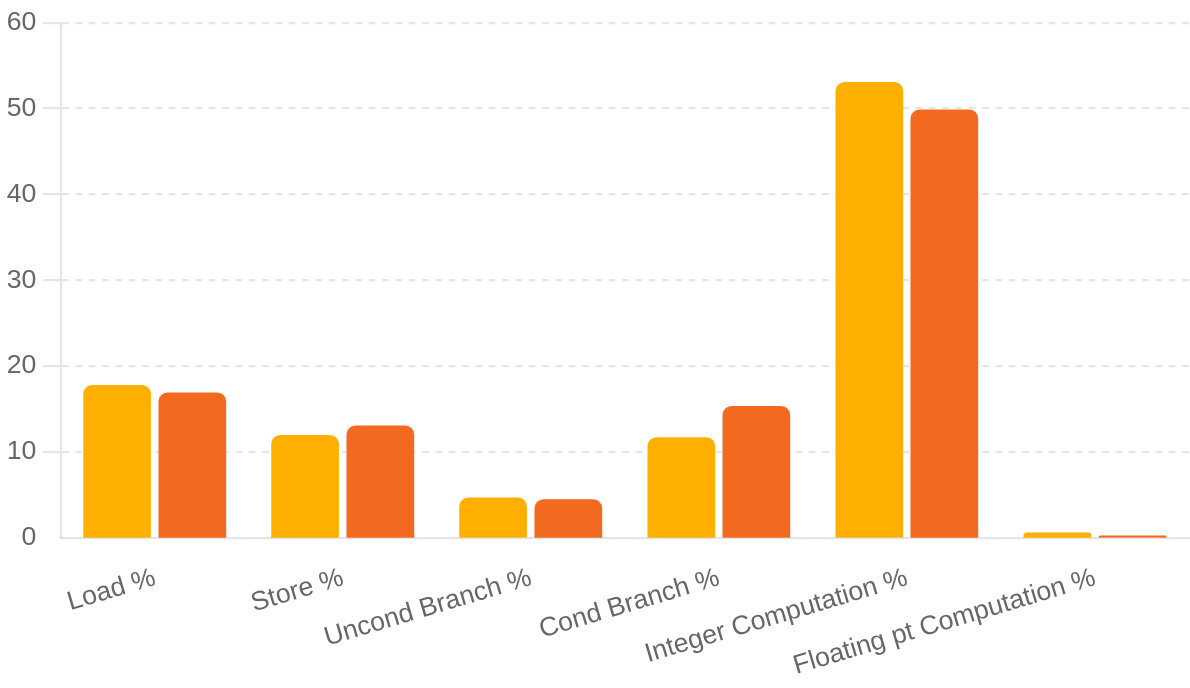
\includegraphics[scale=0.3]{Comparison of Instruction Types Between Alpha and Pisa ISAs.png}
	\caption{Comparison of Instruction Types (Averages) Between Alpha and Pisa ISAs}
	\label{fig:memory_bandwidth}
\end{figure}
Seems like PISA generates a lot more instructions, compared to Alpha, from the compiler, this indicates that the perhaps PISA's MIPs implementation is more CISC like when compared to the Alpha ISA. 

\section{Lab 6}
\subsection{Tests}

\begin{figure}[H]
	\centering
	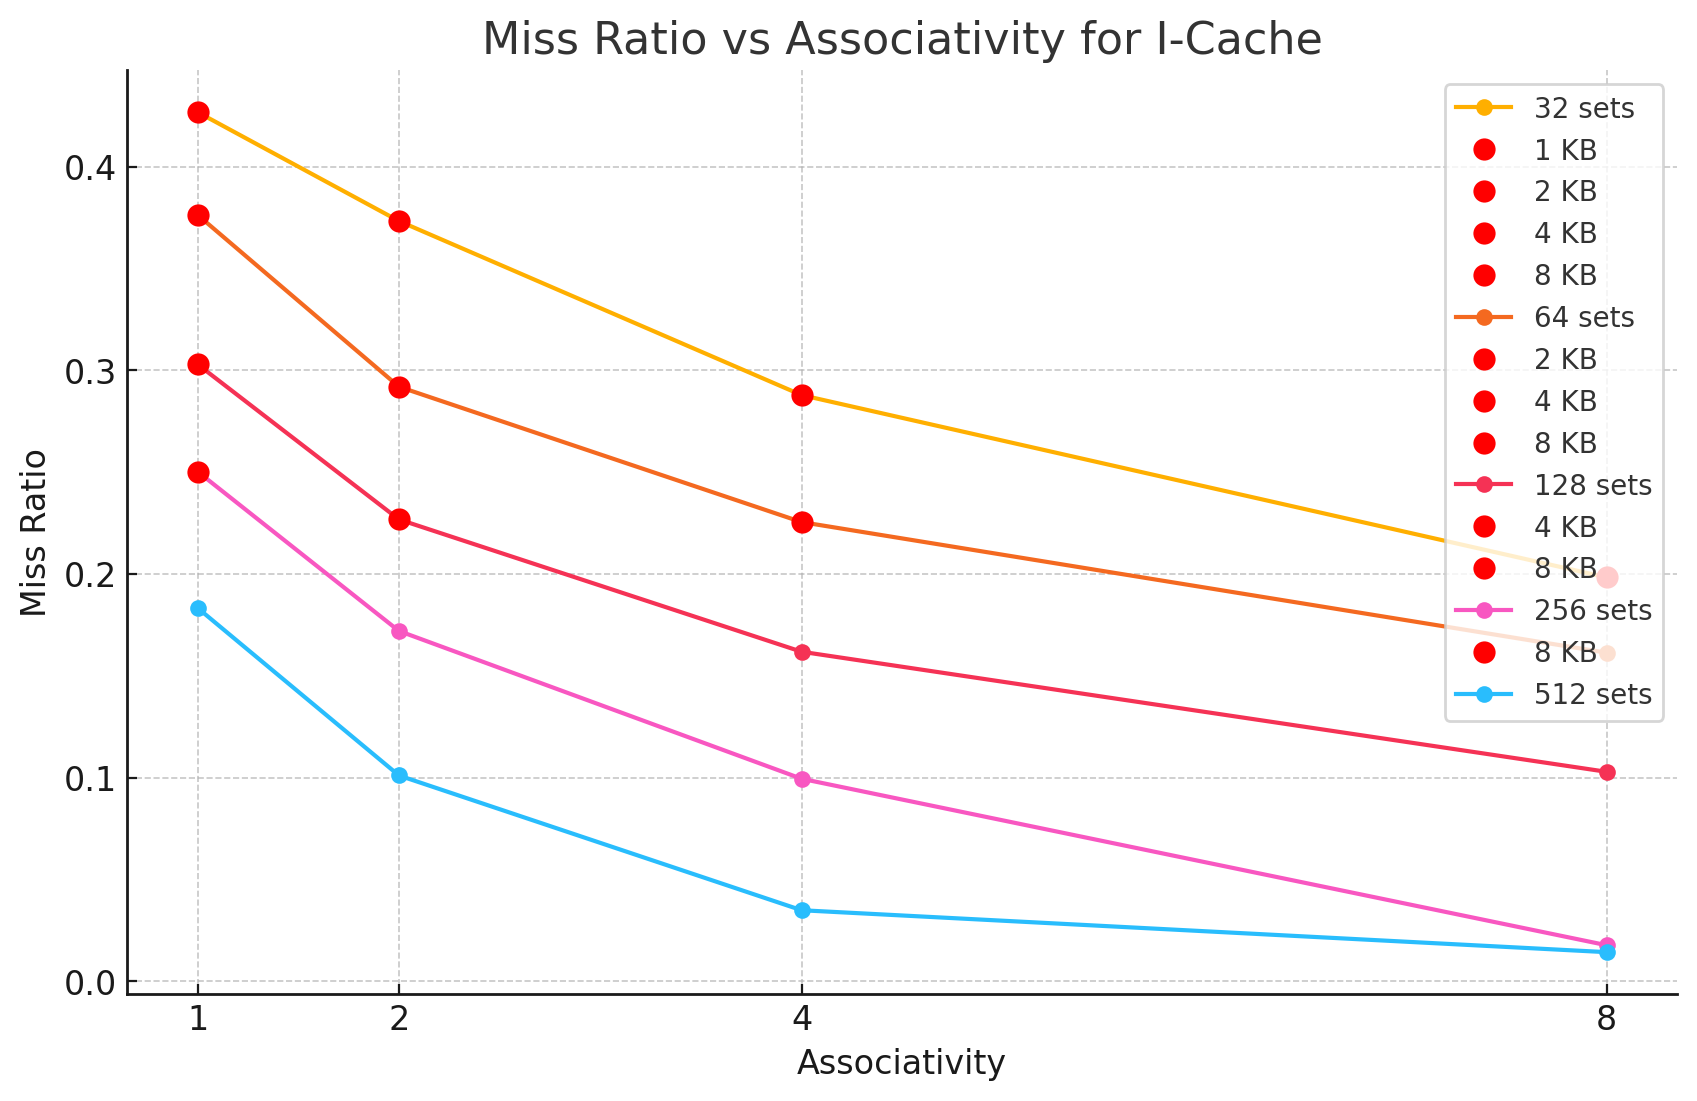
\includegraphics[scale=0.5]{icache.png}
	\caption{Miss Ratio vs Associativity for I-Cache}
	\label{fig:icache}
\end{figure}
\begin{table}[h]
	\centering
	\begin{tabular}{|c|c|c|c|c|}
		\hline
		\textbf{Miss Ratio (I-Cache)} & \textbf{1-way} & \textbf{2-way} & \textbf{4-way} & \textbf{8-way} \\ \hline
		\textbf{32 sets}  &       0.4269      &       0.3734     &      0.2879       &       0.1983      \\ \hline
		\textbf{64 sets}  &        0.3764    &       0.2920     &       0.2255      &      0.1613      \\ \hline
		\textbf{128 sets} &       0.3030      &       0.2268     &        0.1618    &      0.1028       \\ \hline
		\textbf{256 sets} &        0.2503     &      0.1720       &      0.0994       &       0.0176      \\ \hline
		\textbf{512 sets} &       0.1833     &      0.1010      &       0.0348      &      0.0142      \\ \hline
	\end{tabular}
	\caption{Miss Ratio for I-Cache}
	\label{tab:I-Cache}
\end{table}


\begin{figure}[H]
	\centering
	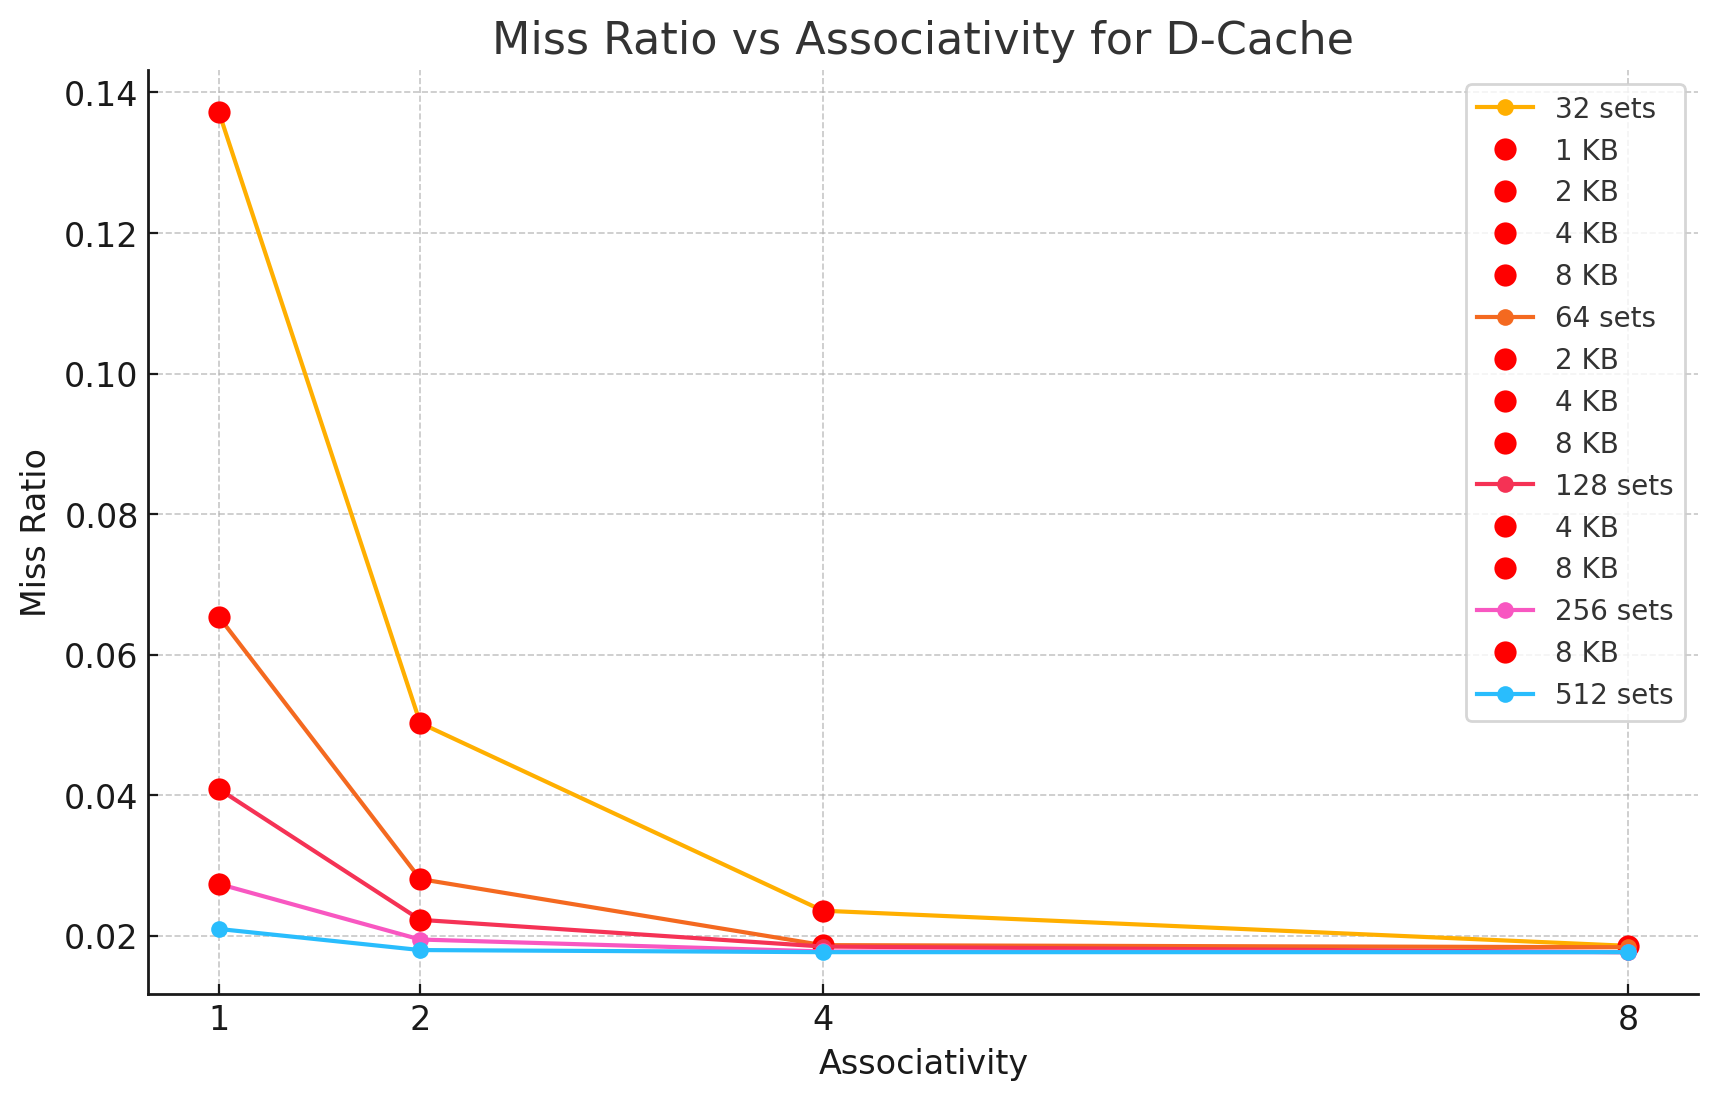
\includegraphics[scale=0.5]{dcache.png}
	\caption{Miss Ratio vs Associativity for D-Cache}
	\label{fig:dcache}
\end{figure}


\begin{table}[h]
	\centering
	\begin{tabular}{|c|c|c|c|c|}
		\hline
		\textbf{Miss Ratio (D-Cache)} & \textbf{1-way} & \textbf{2-way} & \textbf{4-way} & \textbf{8-way} \\ \hline
		\textbf{32 sets}  &       0.1372    &     0.0503       &        0.0236      &     0.0186        \\ \hline
		\textbf{64 sets}  &      0.0654       &      0.0281       &     0.0187       &       0.0184      \\ \hline
		\textbf{128 sets} &      0.0409       &       0.0223      &      0.0185       &      0.0177       \\ \hline
		\textbf{256 sets} &       0.0274      &      0.0195       &      0.0178       &      0.0177        \\ \hline
		\textbf{512 sets} &      0.0210       &      0.0180       &      0.0177       &     0.0177        \\ \hline
	\end{tabular}
	\caption{Miss Ratio for D-Cache}
	\label{tab:D-Cache}
\end{table}

\subsection{Cache Simulation Analysis}

\subsubsection{Questions and Answers}

\textbf{Q1: For a given number of sets, what effect does increasing associativity have on the miss ratio?}

For a given number of sets, increasing associativity reduces the miss ratio. This is evident from the tables where, for each fixed number of sets, the miss ratio decreases as the associativity increases. Higher associativity allows more blocks to be in the same set, reducing conflict misses caused by multiple blocks competing for the same cache location.

\textbf{Q2: For a given associativity, what is the effect of increasing the number of sets?}

For a given associativity, increasing the number of sets decreases the miss ratio. This is because increasing the number of sets effectively enlarges the cache size (since total cache size = number of sets $\times$ associativity $\times$ block size), allowing more unique blocks to be stored. This reduces capacity misses, as the cache can hold more data.

\textbf{Q3: For a given cache size, how does the miss ratio change when going from an associativity of one to two to four? Explain.}

For a given cache size, increasing associativity from one to two to four generally leads to a reduction in the miss ratio, but the improvement diminishes with higher associativity. This is because, while higher associativity reduces conflict misses by allowing more blocks per set, the total number of unique blocks that can be stored (cache capacity) remains the same. Therefore, the initial increase from direct-mapped (1-way) to 2-way associativity shows a noticeable improvement, but going from 2-way to 4-way yields \textit{smaller gains} due to diminishing returns.

\textbf{Q4: If you were to design an Instruction cache, limited to a total cache size of 4 Kbytes, which cache organization would you choose, based solely on performance?}

For designing a 4 Kbytes instruction cache based on performance, the best choice is a \textbf{4-way set-associative cache with 32 sets}. This configuration offers the lowest miss ratio among the options with the same cache size (4 Kbytes). 

\begin{itemize}
	\item Cache size = Number of sets $\times$ Associativity $\times$ Block size
	\item Assuming a block size of 32 bytes, the configurations that yield 4 Kbytes cache size are:
	\begin{itemize}
		\item 1-way, 128 sets
		\item 2-way, 64 sets
		\item 4-way, 32 sets
	\end{itemize}
	\item From the I-Cache table:
	\begin{itemize}
		\item 1-way, 128 sets: miss ratio = 0.3030
		\item 2-way, 64 sets: miss ratio = 0.2920
		\item \textbf{4-way, 32 sets: miss ratio = 0.2879 (lowest)}
	\end{itemize}
\end{itemize}

\textbf{Q5: If you were to design a data cache, limited to a total cache size of 4 Kbytes, which cache organization would you choose, based solely on performance?}

For designing a 4 Kbytes data cache based on performance, the optimal choice is a \textbf{4-way set-associative cache with 32 sets}. This configuration provides the lowest miss ratio among the available options with the same cache size. Supporting data:

\begin{itemize}
	\item Cache size = Number of sets $\times$ Associativity $\times$ Block size
	\item Assuming a block size of 32 bytes, the configurations that yield 4 Kbytes cache size are:
	\begin{itemize}
		\item 1-way, 128 sets
		\item 2-way, 64 sets
		\item 4-way, 32 sets
	\end{itemize}
	\item From the D-Cache table:
	\begin{itemize}
		\item 1-way, 128 sets: miss ratio = 0.0409
		\item 2-way, 64 sets: miss ratio = 0.0281
		\item \textbf{4-way, 32 sets: miss ratio = 0.0236 (lowest)}
	\end{itemize}
\end{itemize}

\section{Problem 2}
\subsection{Assignment 1}
\begin{enumerate}
	\item What are the four main categories of cache performance optimizations? Relate these to the
	formula for average memory access time.
	\begin{itemize}
		\item The goal of cache performance optimizations is to improve hit rate, reduce the miss rate, being able to make the miss penalty as few clock cycles as possible, and miss rate via parallelism. The formula for AMAT directly includes all of these variables, and thus optimizing these variables directly influences the memory access speed of the system. The specific optimizations are the number of associative sets, larger block sizes, a larger cache, and utilizing better cache replacement algorithms.  
	\end{itemize}
	\item Which of these categories does associativity affect?
	\begin{itemize}
		\item Increasing the associativity of a cache reduces the number of conflict misses by allowing a block to be placed in multiple locations. This enhancement decreases the overall miss rate, directly impacting the Miss Rate term in the AMAT formula.
	\end{itemize}
	\item Which of these categories does block size affect?
	\begin{itemize}
		\item A larger block size can reduce the miss rate by fetching adjacent data that is likely to be accessed soon (spatial locality), thus decreasing compulsory misses. However, a larger block size can increase the miss penalty because it takes longer to transfer a bigger block of data from the next level in the memory hierarchy.
	\end{itemize}
\end{enumerate}
\subsection{Assignment 2}
\begin{enumerate}
	\item How is associativity, number of blocks, number of sets and cache size related?
	\begin{itemize}
		\item Associativity determines how many blocks can be in a single set. Higher associativity means more blocks per set.
		\item The number of blocks is the total storage capacity divided by the block size.
		\item The number of sets is influenced by both the total number of blocks and the associativity.
		\item Cache Size depends on the block size, number of sets, and associativity.
	\end{itemize}
	\item How does these affect the average access time for L1- and L2-caches?
	\begin{itemize}
		\item For an L1 cache: Prioritizes low hit time over miss rate.
		\begin{enumerate}
			\item  Increasing associativity will increase the complexity of the hardware, increasing the hit time; higher associativity reduces conflict misses, lowering the miss rate. L1 caches need low access times however, since it is the first memory outside of registers that the CPU accesses so it makes sense that the associativity for the L1 might be low.
			\item Increasing the number of blocks (and thus cache size) can increase the hit time due to longer access times from a larger block size; a larger cache size reduces the miss rate by storing and receiving more data on each transaction from the cache. An L1 cache is kept small on purpose, in order to have low access times to the CPU.
			\item Increasing the number of sets (while maintaining cache size) reduces the associativity, increasing the number of conflict misses, raising the miss rate; an increased number of sets means that less collisions happen in cache, decreasing the number of conflict misses. However, if we increase the number of sets while increasing the size of cache, we reduce the conflict misses overall; the complexity of the hardware is dramatically increased, as a wider comparison would have to happen over the whole cache, increasing hit times. It makes sense for an L1 cache to have a lower number of sets to maximize the AMAT.  
		\end{enumerate}
		\item For an L2 cache: Prioritizes low miss rate over hit time.
		\begin{enumerate}
			\item  L2 caches can afford a slightly higher hit time because they are not accessed as frequently as L1 caches; Higher associativity reduces the miss rate, which is crucial for L2 caches to prevent slower main memory accesses. An L2 cache would have a high associativity, slowing down the hit time, but decreasing the miss rate, since L2 is not accessed as frequently as L1. 
			\item Increasing the number of blocks can increase the hit time due to longer access times; a larger cache size reduces the miss rate by storing more data on each transaction. L2 caches are designed to be larger to reduce miss rates, with a higher hit time.
			\item A higher set size while increasing the size of cache, increases the hit time as a larger comparison would have to happen across the cache; a higher set size means miss rate is reduced by reducing conflict misses.
		\end{enumerate}
	\end{itemize}
\end{enumerate}
\newpage
\subsection{Deliverable 1}
\textbf{Using sim-cache \& test-math for Cache sizes of 32 KB, 16 KB, and 8 KB}
\begin{table}[h!]
	\centering
	\begin{tabular}{ccc}
		\toprule
		\textbf{Associativity} & \textbf{Number of Sets} & \textbf{Unified Cache Miss Rate (\%)} \\
		\midrule
		1-way  & 1024 &  0.0372  \\
		2-way  & 512  &   0.0238 \\
		4-way  & 256  &  0.0209  \\
		8-way  & 128  &   0.0204 \\
		\midrule
		1-way  & 512  &   0.0584 \\
		2-way  & 256  &   0.0449 \\
		4-way  & 128  &   0.0283 \\
		8-way  & 64   &   0.0233 \\
		\midrule
		1-way  & 256  &    0.0967\\
		2-way  & 128  &    0.0789\\
		4-way  & 64   &    0.0742\\
		8-way  & 32   &    0.0766\\
		\bottomrule
	\end{tabular}
	\caption{Unified Cache Simulation Results}
\end{table}
\begin{figure}[H]
	\centering
	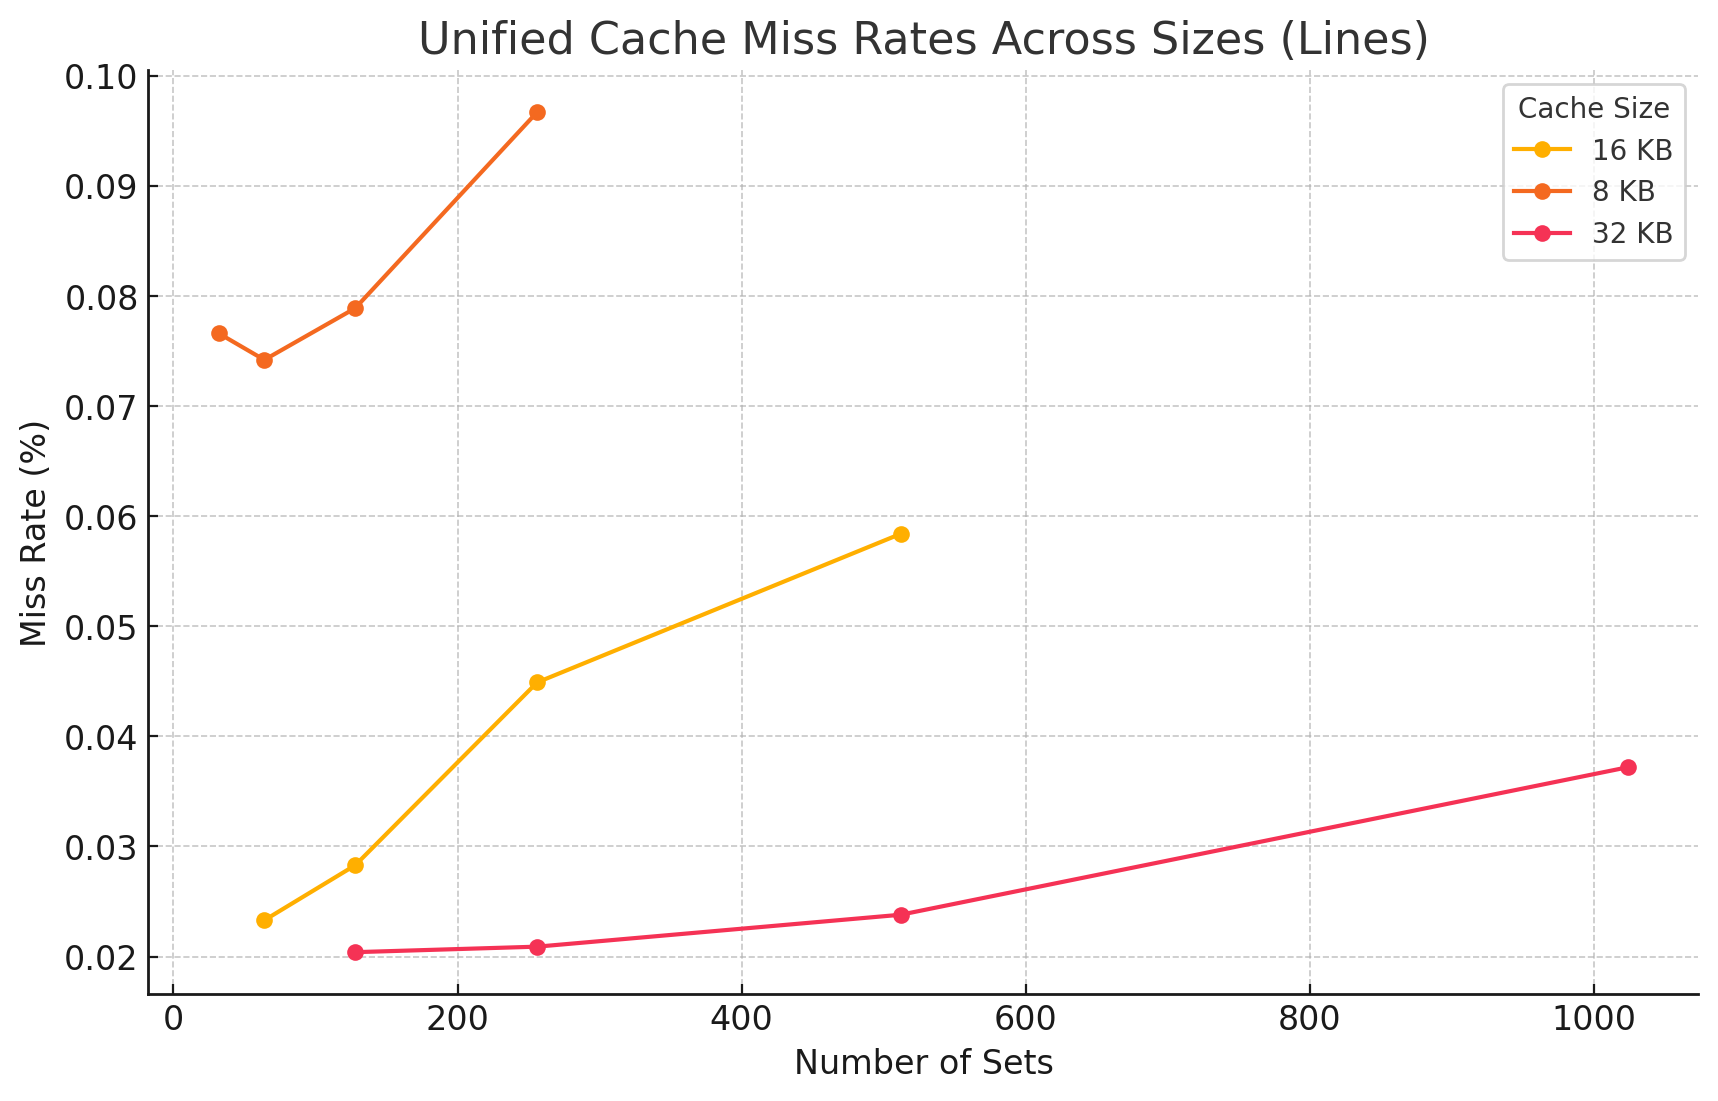
\includegraphics[scale=0.5]{deliv1_unified.png}
	\caption{Unified cache miss rate}
	\label{fig:Unifed Cache Results}
\end{figure}
\begin{table}[h!]
	\centering
	\begin{tabular}{ccc}
		\toprule
		\textbf{Associativity} & \textbf{Number of Sets} & \textbf{Instruction Cache Miss Rate (\%)} \\
		\midrule
		1-way  & 1024 &   0.0330 \\
		2-way  & 512  &    0.0200\\
		4-way  & 256  &    0.0185\\
		8-way  & 128  &   0.0178 \\
		\midrule
		1-way  & 512  &    0.0527\\
		2-way  & 256  &    0.0398\\
		4-way  & 128  &   0.0220\\
		8-way  & 64   &   0.0194\\
		\midrule
		1-way  & 256  &    0.0898\\
		2-way  & 128  &    0.0673\\
		4-way  & 64   &    0.0615\\
		8-way  & 32   &    0.0527\\
		\bottomrule
	\end{tabular}
	\caption{Instruction Cache Simulation Results}
\end{table}
\begin{figure}[H]
	\centering
	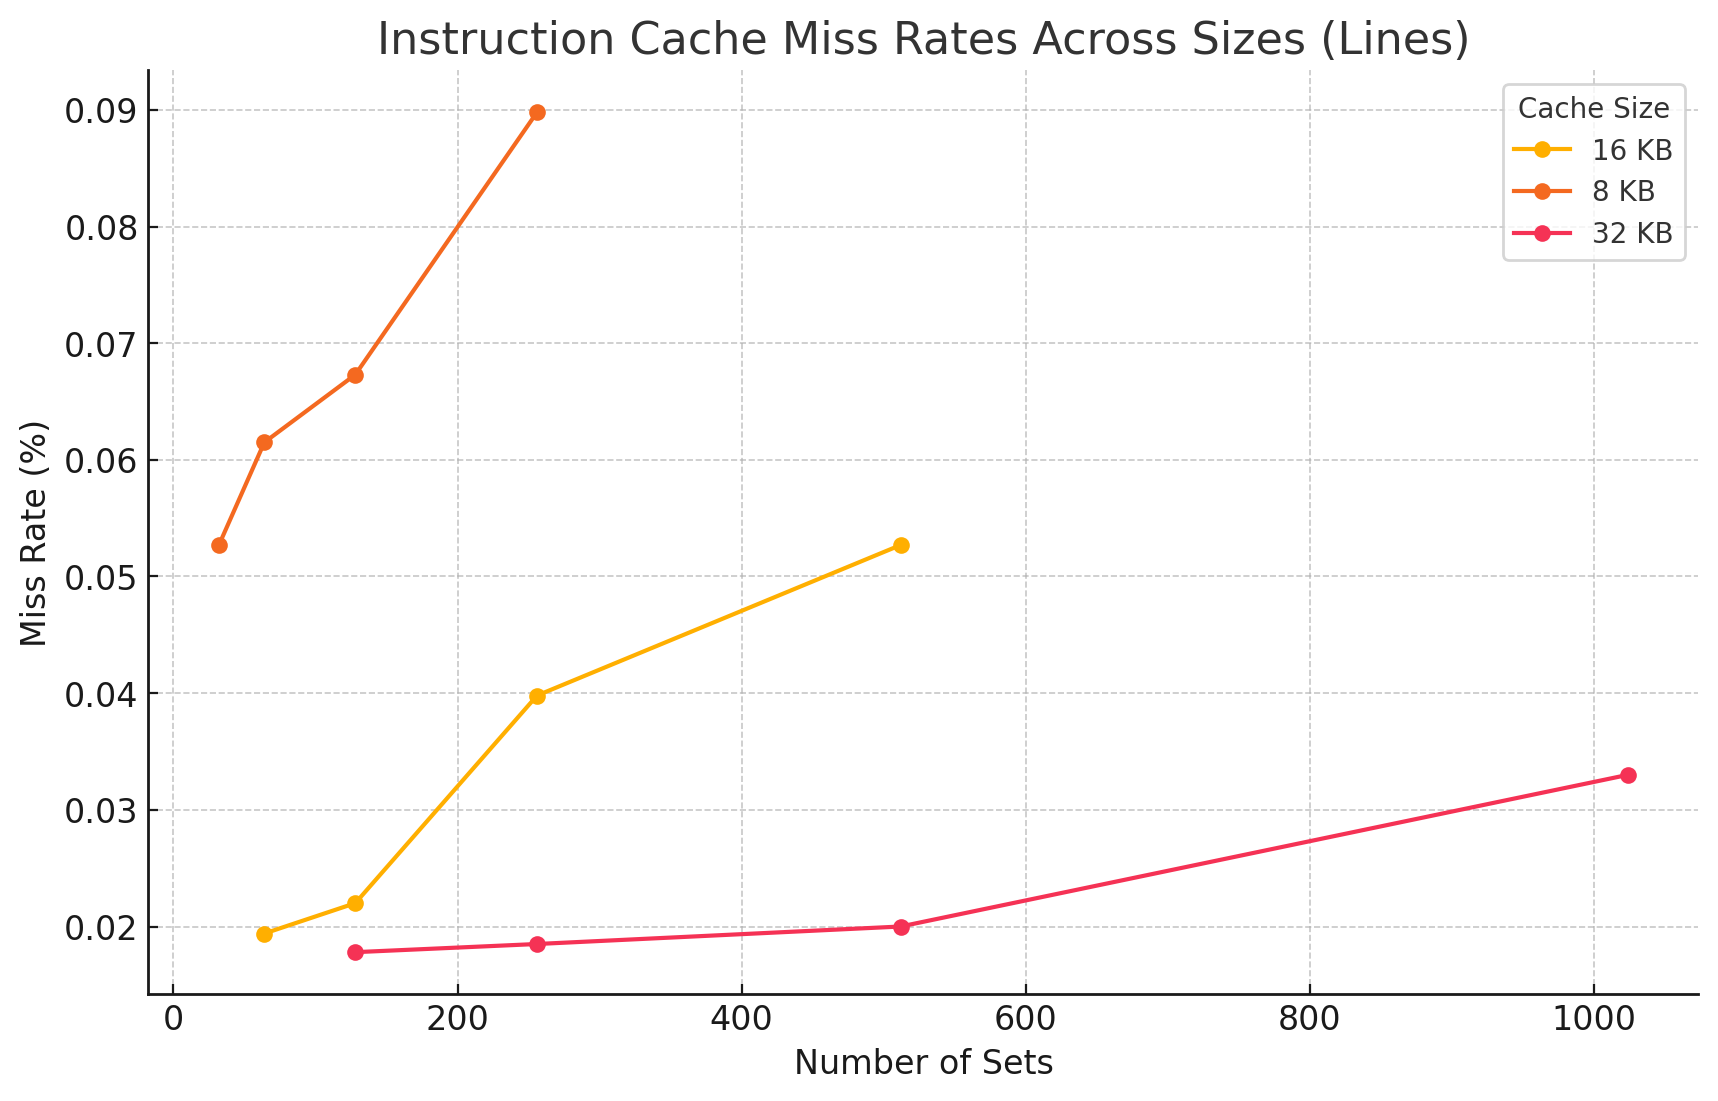
\includegraphics[scale=0.5]{deliv1_instruction.png}
	\caption{Instruction cache miss rate}
	\label{fig:Instruction Cache Results}
\end{figure}
\begin{table}[h!]
	\centering
	\begin{tabular}{ccc}
		\toprule
		\textbf{Associativity} & \textbf{Number of Sets} & \textbf{Data Cache Miss Rate (\%)} \\
		\midrule
		1-way  & 1024 &    0.0329\\
		2-way  & 512  &    0.0282\\
		4-way  & 256  &    0.0275\\
		8-way  & 128  &    0.0275\\
		\midrule
		1-way  & 512  &    0.0422\\
		2-way  & 256  &    0.0296\\
		4-way  & 128  &   0.0276\\
		8-way  & 64   &   0.0275\\
		\midrule
		1-way  & 256  &    0.0501\\
		2-way  & 128  &    0.0341\\
		4-way  & 64   &    0.0298\\
		8-way  & 32   &    0.0292\\
		\bottomrule
	\end{tabular}
	\caption{Data Cache Simulation Results}
\end{table}
\begin{figure}[H]
	\centering
	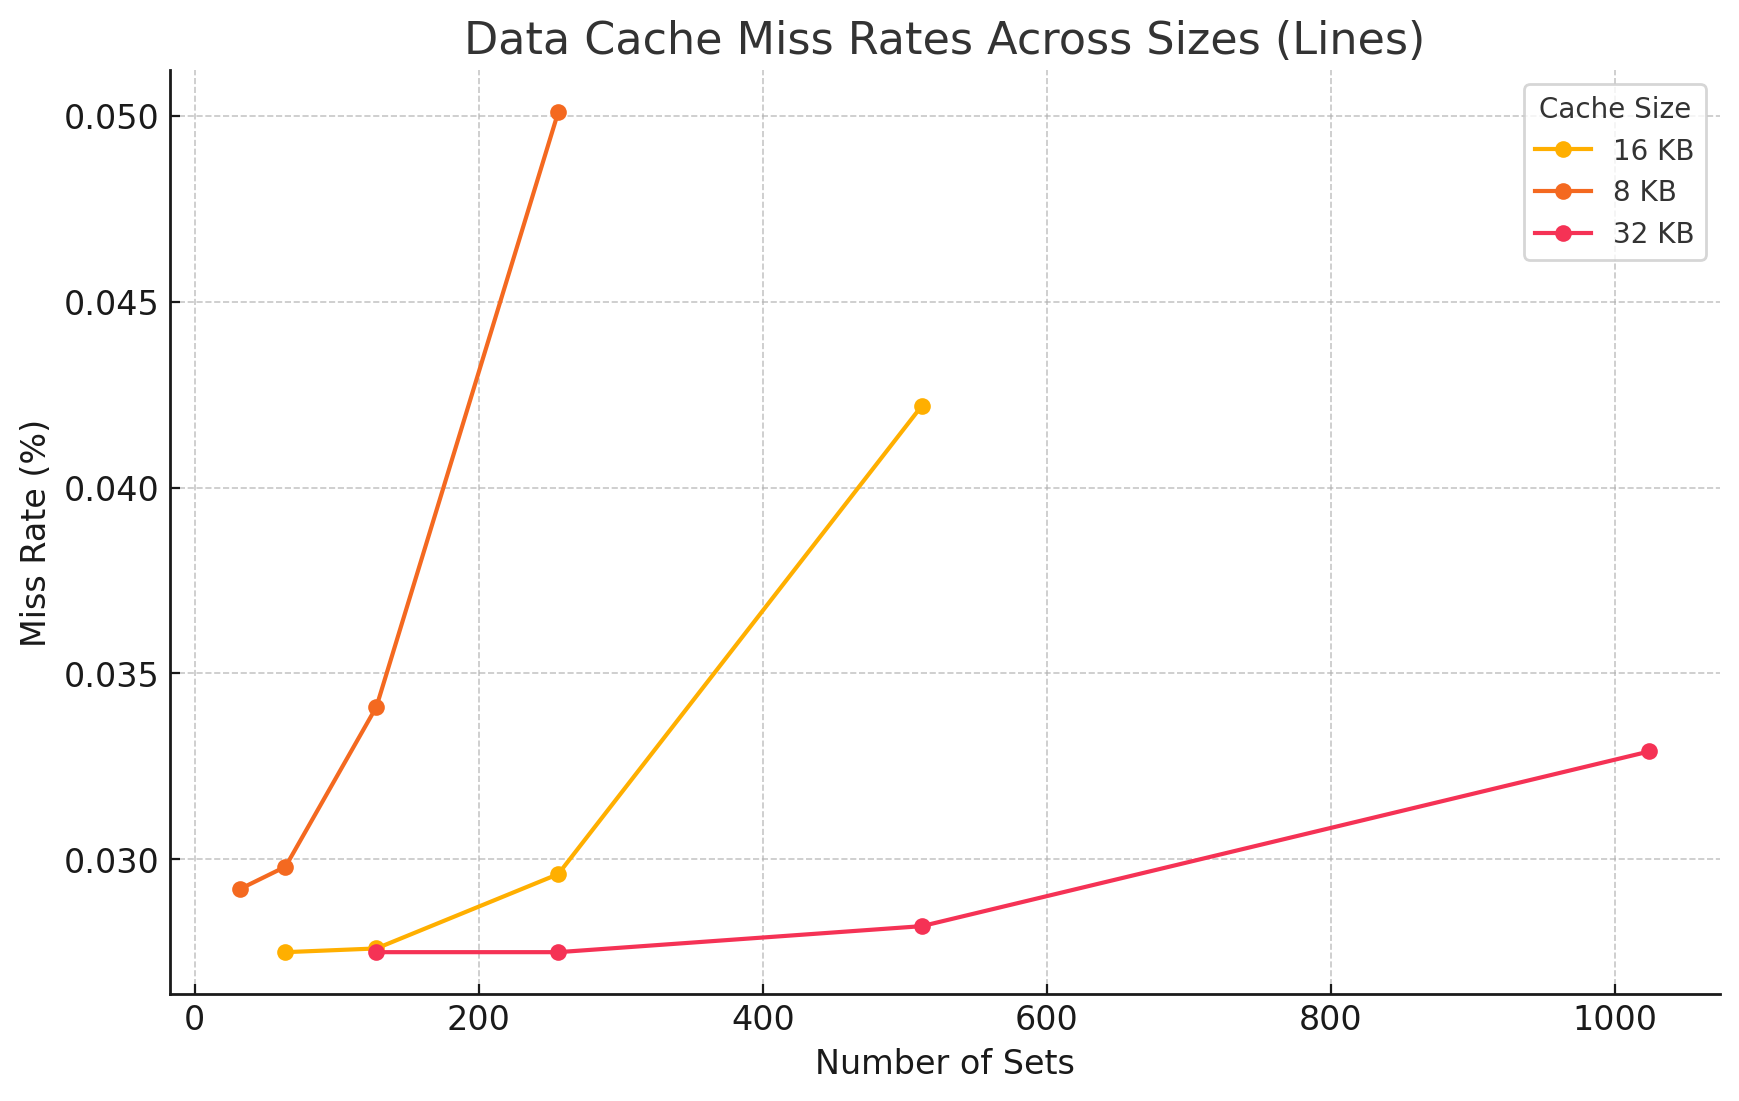
\includegraphics[scale=0.5]{deliv_data.png}
	\caption{Data cache miss rate}
	\label{fig:Data Cache Results}
\end{figure}
\newpage
\subsection{Deliverable 2}
\begin{table}[h!]
	\centering
	\begin{tabular}{|c|c|c|c|}
		\hline
		\multicolumn{4}{|c|}{L2 data cache} \\
		\hline
		fixed total size & No of sets & block size ($\geq$ 256) & associativity \\
		\hline
		512 KB & 128 & 512 & 8\\
		\hline
	\end{tabular}
	\caption{L2 Data Cache}
\end{table}

\begin{table}[h!]
	\centering
	\begin{tabular}{|c|c|c|c|c|c|}
		\hline
		L1 size & L1 assoc & No of sets & block size & CPI & Average Memory Access Time (cycles) \\
		\hline
		32 KB & 2 & 1024 & 16 &  1.0395& 6.2\\
		32 KB & 2 & 512& 32 &  0.9646& 5.16\\
		32 KB & 2 & 256& 64 & 0.9253 & 4.64\\
		32 KB & 2 & 128& 128 &  0.9107& 4.12\\
		32 KB & 2 & 64& 256 & 0.9157 & 4.328\\
		\hline
	\end{tabular}
	\caption{L1 Data Cache}
\end{table}
\begin{figure}[H]
	\centering
	\begin{minipage}{0.48\textwidth}
		\centering
		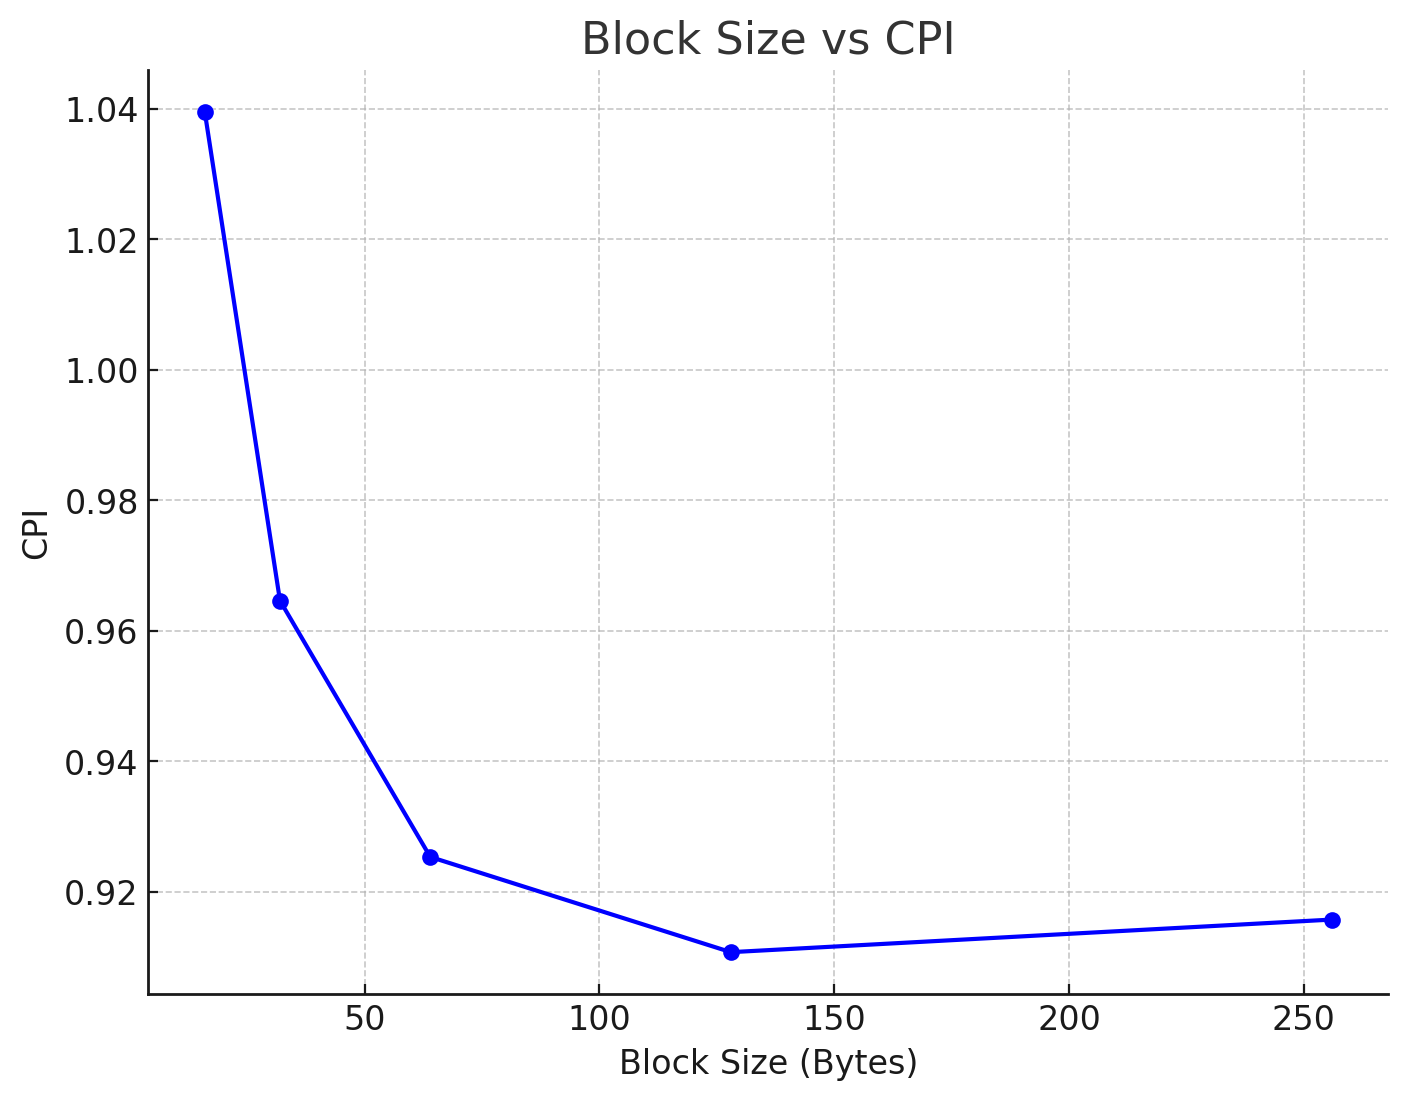
\includegraphics[scale=0.5]{block_cpi.png}
		\caption{Block size vs CPI}
		\label{fig:block vs cpi}
	\end{minipage}
	\hfill
	\begin{minipage}{0.48\textwidth}
		\centering
		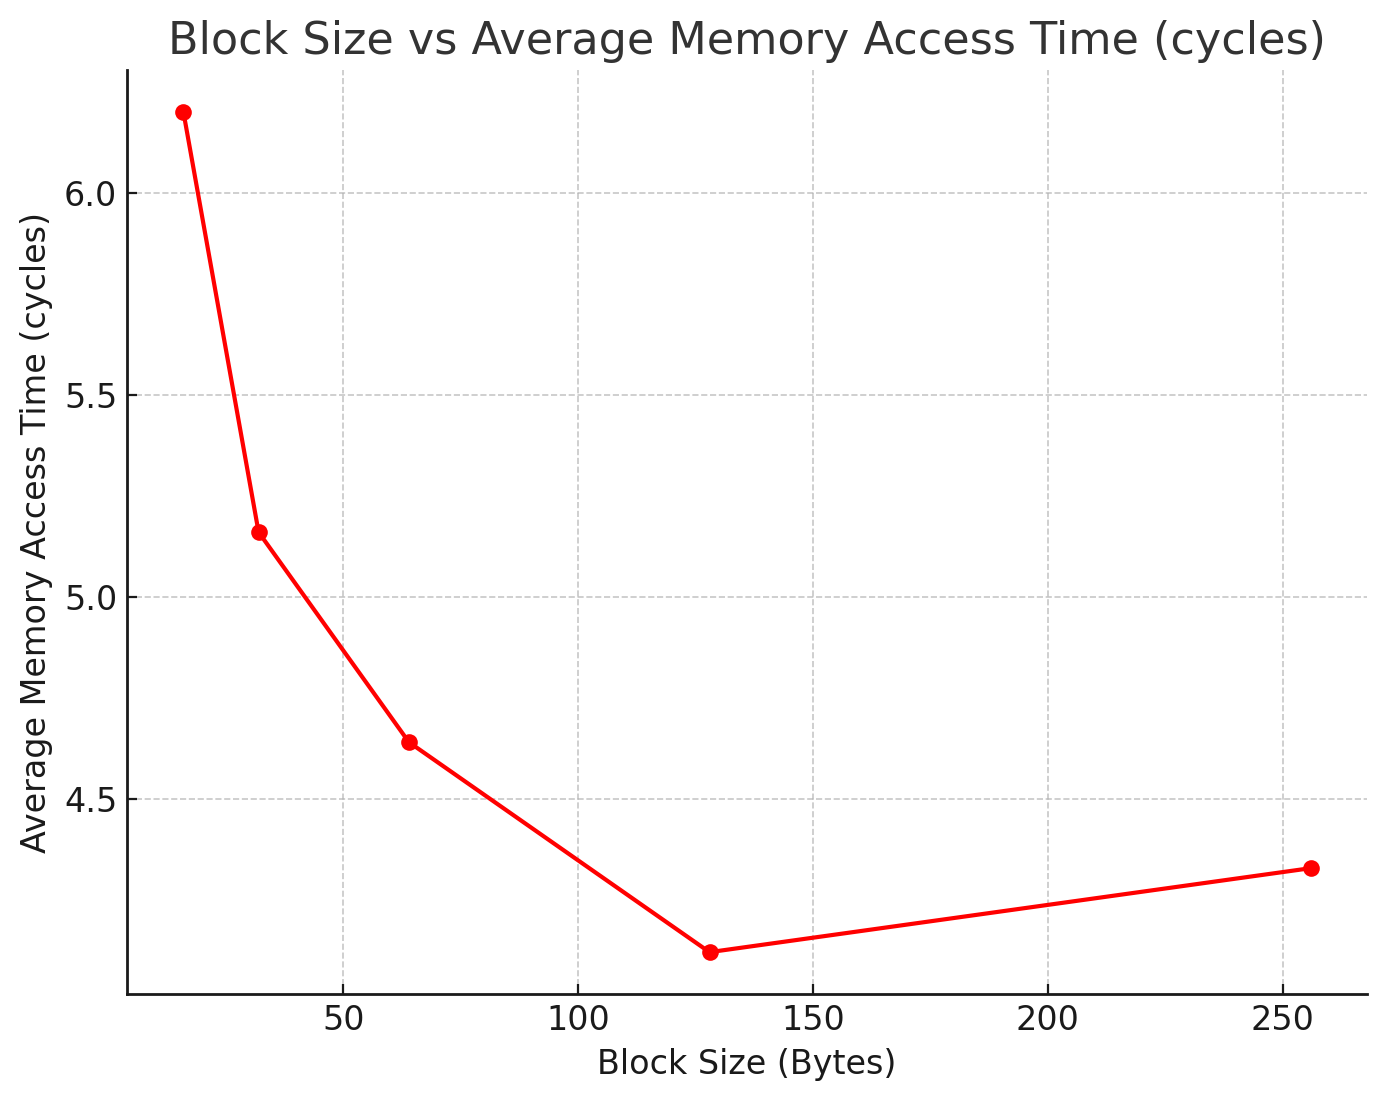
\includegraphics[scale=0.5]{block_amat.png}
		\caption{Block size vs AMAT}
		\label{fig:block vs AMAT}
	\end{minipage}
\end{figure}



	
\end{document}
